\documentclass[12pt, a4paper]{article}

% ─── Packages ────────────────────────────────────────────
\usepackage[margin=1in, headheight=15pt]{geometry}
\usepackage{amsmath, amssymb}
\usepackage{graphicx}
\usepackage{xcolor}
\usepackage{booktabs}
\usepackage{array}
\usepackage{multirow}
\usepackage{pifont}
\usepackage{enumitem}
\usepackage{tikz}
\usetikzlibrary{automata, positioning, arrows.meta, calc, shapes.geometric, decorations.pathmorphing}
\usepackage{circuitikz}
\usepackage{hyperref}
\usepackage{tcolorbox}
\usepackage{fancyhdr}
\usepackage{titlesec}
\usepackage{float}

% ─── Colors ──────────────────────────────────────────────
\definecolor{primary}{HTML}{1A5276}
\definecolor{accent}{HTML}{2E86C1}
\definecolor{highlight}{HTML}{E74C3C}
\definecolor{success}{HTML}{27AE60}
\definecolor{bg}{HTML}{F0F4F8}
\definecolor{statebg}{HTML}{D6EAF8}

% ─── tcolorbox styles ───────────────────────────────────
\tcbuselibrary{skins, breakable}

\newtcolorbox{keypoint}[1][]{
  colback=blue!5, colframe=primary, 
  fonttitle=\bfseries, title=#1,
  sharp corners, boxrule=1pt, breakable
}

\newtcolorbox{important}[1][]{
  colback=red!5, colframe=highlight, 
  fonttitle=\bfseries, title=#1,
  sharp corners, boxrule=1.5pt, breakable
}

\newtcolorbox{tip}[1][]{
  colback=green!5, colframe=success, 
  fonttitle=\bfseries, title=#1,
  sharp corners, boxrule=1pt, breakable
}

% ─── Header/Footer ──────────────────────────────────────
\pagestyle{fancy}
\fancyhf{}
\fancyhead[L]{\textcolor{primary}{\textbf{FSM Design Guide}}}
\fancyhead[R]{\textcolor{primary}{DSD -- Chapter 3}}
\fancyfoot[C]{\thepage}
\renewcommand{\headrulewidth}{1pt}
\renewcommand{\headrule}{\hbox to\headwidth{\color{primary}\leaders\hrule height \headrulewidth\hfill}}

% ─── Section Formatting ─────────────────────────────────
\titleformat{\section}{\Large\bfseries\color{primary}}{}{0em}{\thesection\quad}[\color{primary}\titlerule]
\titleformat{\subsection}{\large\bfseries\color{accent}}{}{0em}{\thesubsection\quad}

% ─── TikZ Styles ────────────────────────────────────────
\tikzset{
  fsm state/.style={
    state, 
    draw=primary, 
    very thick, 
    fill=statebg,
    minimum size=1.3cm,
    font=\footnotesize\bfseries,
    align=center,
    text width=1.2cm,
    inner sep=3pt
  },
  fsm arrow/.style={
    -Stealth, 
    thick, 
    color=primary
  },
  initial text={},
  every initial by arrow/.style={fsm arrow},
  block/.style={
    draw=primary, thick, fill=statebg,
    minimum width=2.5cm, minimum height=1.5cm,
    align=center, font=\small
  },
  register/.style={
    draw=primary, thick, fill=blue!10,
    minimum width=2.5cm, minimum height=0.8cm,
    align=center, font=\small
  },
  io/.style={-Stealth, thick, color=primary},
  clk/.style={-Stealth, thick, color=highlight}
}

% ─── Document ────────────────────────────────────────────
\begin{document}

% ═══════════════════════════════════════════════════════
% TITLE PAGE
% ═══════════════════════════════════════════════════════
\begin{titlepage}
\centering
\vspace*{2cm}

{\Huge\bfseries\color{primary} Finite-State Machine (FSM)\\[6pt] Design Guide}

\vspace{0.5cm}
{\Large\color{accent} A Complete Learning Reference}

\vspace{1.5cm}

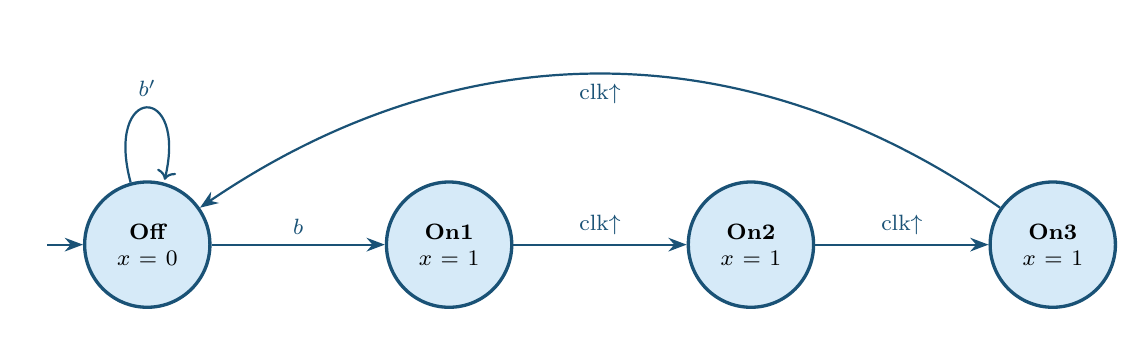
\begin{tikzpicture}[node distance=2.2cm]
  \node[fsm state, initial] (off) {Off \\ \footnotesize $x=0$};
  \node[fsm state, right=of off] (on1) {On1 \\ \footnotesize $x=1$};
  \node[fsm state, right=of on1] (on2) {On2 \\ \footnotesize $x=1$};
  \node[fsm state, right=of on2] (on3) {On3 \\ \footnotesize $x=1$};
  
  \draw[fsm arrow] (off) edge[loop above] node[above]{\footnotesize $b'$} (off);
  \draw[fsm arrow] (off) -- node[above]{\footnotesize $b$} (on1);
  \draw[fsm arrow] (on1) -- node[above]{\footnotesize clk$\uparrow$} (on2);
  \draw[fsm arrow] (on2) -- node[above]{\footnotesize clk$\uparrow$} (on3);
  \draw[fsm arrow] (on3) to[bend right=35] node[below]{\footnotesize clk$\uparrow$} (off);
\end{tikzpicture}

\vspace{1.5cm}

{\large Based on \textit{Digital Design} by Frank Vahid --- Chapter 3, Part 2}

\vspace{0.5cm}
{\large Sequential Logic Design: Controllers}

\vfill
{\color{gray}\today}
\end{titlepage}

% ═══════════════════════════════════════════════════════
% TABLE OF CONTENTS
% ═══════════════════════════════════════════════════════
\tableofcontents
\newpage

% ═══════════════════════════════════════════════════════
% SECTION 1: WHY FSMs?
% ═══════════════════════════════════════════════════════
\section{Why Do We Need FSMs?}

\subsection{The Problem with Trial-and-Error}

When designing \textbf{combinational circuits}, engineers have:
\begin{enumerate}
  \item A \textbf{formal way} to describe behavior --- Boolean equations or truth tables
  \item A \textbf{well-defined process} to convert that behavior into a circuit
\end{enumerate}

But for \textbf{sequential circuits} (circuits with memory/state), no such formal tool existed in our discussion --- until now.

\begin{important}[Why Trial-and-Error Fails]
  \textbf{Example:} You need a laser timer with output $x=1$ for exactly 3 clock cycles after a button press.
  \begin{itemize}
    \item Can you ``guess'' a circuit? Maybe with 3 flip-flops and an OR gate\ldots
    \item But what if someone presses the button \textbf{again} while $x=1$?
    \item What about circuits with 9 states? 100 states?
    \item A guessed circuit may have \textbf{undesired behavior} that's hard to detect.
  \end{itemize}
  \textbf{Solution:} We need \textbf{FSMs} --- a formal mathematical model for sequential behavior.
\end{important}

% ═══════════════════════════════════════════════════════
% SECTION 2: WHAT IS AN FSM?
% ═══════════════════════════════════════════════════════
\section{What is a Finite-State Machine (FSM)?}

\begin{keypoint}[Definition]
  An FSM is a mathematical model that describes sequential circuit behavior by listing all possible \textbf{states} and the \textbf{transitions} between them, triggered by inputs and clock edges.
\end{keypoint}

\subsection{The 5 Components of Every FSM}

\begin{table}[H]
\centering
\renewcommand{\arraystretch}{1.4}
\begin{tabular}{@{} >{\bfseries}l c p{7.5cm} @{}}
  \toprule
  Component & Symbol & Description \\
  \midrule
  States       & $\bigcirc$ & All possible conditions the machine can be in \\
  Inputs       & $b, x, \ldots$   & External signals that affect transitions \\
  Outputs      & $x, L, \ldots$   & Signals produced in each state \\
  Transitions  & $\rightarrow$    & Rules for moving from one state to another \\
  Initial State & $\rightarrow\!\bigcirc$ & The state on power-up (arrow from nowhere) \\
  \bottomrule
\end{tabular}
\caption{Five components of a Finite-State Machine}
\end{table}

\begin{tip}[State Count \& Flip-Flop Count]
  $n$ flip-flops $\Rightarrow$ $2^n$ possible states.\\[4pt]
  \begin{tabular}{@{} c c @{\hspace{2cm}} c c @{}}
    States & Flip-Flops & States & Flip-Flops \\
    \cmidrule(r){1-2} \cmidrule(l){3-4}
    2 & 1 & 5--8 & 3 \\
    3--4 & 2 & 9--16 & 4 \\
  \end{tabular}\\[4pt]
  Formula: \ $\text{Flip-flops needed} = \lceil \log_2(\text{\# states}) \rceil$
\end{tip}

% ═══════════════════════════════════════════════════════
% SECTION 3: SIMPLE TOGGLE EXAMPLE
% ═══════════════════════════════════════════════════════
\section{Example 1 --- Simple Toggle}

\subsection{Problem}
Design a circuit whose output $x$ \textbf{toggles} (switches between 0 and 1) on every rising clock edge.

\subsection{FSM State Diagram}

\begin{figure}[H]
\centering
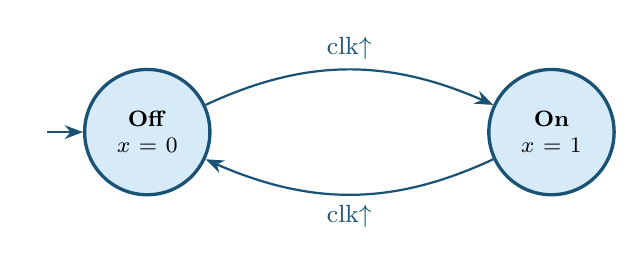
\begin{tikzpicture}[node distance=3.5cm]
  \node[fsm state, initial] (off) {\textbf{Off} \\ $x=0$};
  \node[fsm state, right=of off] (on) {\textbf{On} \\ $x=1$};
  
  \draw[fsm arrow] (off) to[bend left=25] node[above]{\small clk$\uparrow$} (on);
  \draw[fsm arrow] (on) to[bend left=25] node[below]{\small clk$\uparrow$} (off);
\end{tikzpicture}
\caption{FSM for a simple toggle circuit}
\end{figure}

\subsection{Transition Table}

\begin{table}[H]
\centering
\renewcommand{\arraystretch}{1.3}
\begin{tabular}{@{} c c c c @{}}
  \toprule
  Current State & Clock Edge & Next State & Output $x$ \\
  \midrule
  Off & Rising $\uparrow$ & On & $0 \to 1$ \\
  On  & Rising $\uparrow$ & Off & $1 \to 0$ \\
  \bottomrule
\end{tabular}
\end{table}

\begin{itemize}
  \item Only \textbf{2 states} $\Rightarrow$ need \textbf{1 flip-flop} ($2^1 = 2$)
  \item Output $x$ simply equals the state bit $s_0$
  \item Boolean equation: $x = s_0$, \ $n_0 = s_0'$ (complement --- toggle)
\end{itemize}

% ═══════════════════════════════════════════════════════
% SECTION 4: THREE-CYCLES-HIGH LASER TIMER
% ═══════════════════════════════════════════════════════
\section{Example 2 --- Three-Cycles-High Laser Timer (Full Walkthrough)}

\subsection{Problem Statement}

\begin{keypoint}[Laser Timer Problem]
  A patient lies under a laser and presses button $b$. The laser ($x$) must turn \textbf{ON} for \textbf{exactly 3 clock cycles}, then turn OFF. It stays off until $b$ is pressed again.
  
  \textbf{Inputs:} $b$ (button) \quad \textbf{Outputs:} $x$ (laser)
\end{keypoint}

\subsection{Step 1: Identify the States}

\begin{table}[H]
\centering
\renewcommand{\arraystretch}{1.3}
\begin{tabular}{@{} >{\bfseries}c l c @{}}
  \toprule
  State & Meaning & Output $x$ \\
  \midrule
  Off & Laser is off, waiting for button & 0 \\
  On1 & Laser on --- 1st cycle & 1 \\
  On2 & Laser on --- 2nd cycle & 1 \\
  On3 & Laser on --- 3rd cycle & 1 \\
  \bottomrule
\end{tabular}
\caption{States for the three-cycles-high laser timer}
\end{table}

\subsection{Step 2: Draw the FSM State Diagram}

\begin{figure}[H]
\centering
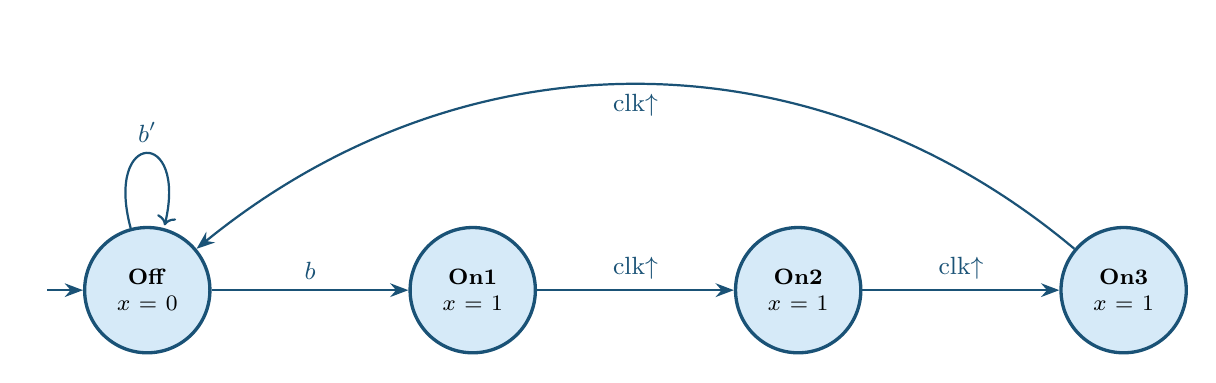
\begin{tikzpicture}[node distance=2.5cm]
  % States
  \node[fsm state, initial] (off) {\textbf{Off} \\ $x=0$};
  \node[fsm state, right=of off] (on1) {\textbf{On1} \\ $x=1$};
  \node[fsm state, right=of on1] (on2) {\textbf{On2} \\ $x=1$};
  \node[fsm state, right=of on2] (on3) {\textbf{On3} \\ $x=1$};
  
  % Transitions
  \draw[fsm arrow] (off) edge[loop above] node[above]{\small $b'$} (off);
  \draw[fsm arrow] (off) -- node[above]{\small $b$} (on1);
  \draw[fsm arrow] (on1) -- node[above]{\small clk$\uparrow$} (on2);
  \draw[fsm arrow] (on2) -- node[above]{\small clk$\uparrow$} (on3);
  \draw[fsm arrow] (on3) to[bend right=40] node[below]{\small clk$\uparrow$} (off);
\end{tikzpicture}
\caption{FSM state diagram for the three-cycles-high laser timer}
\label{fig:laser-fsm}
\end{figure}

\subsection{Cycle-by-Cycle Operation}

\begin{table}[H]
\centering
\renewcommand{\arraystretch}{1.3}
\begin{tabular}{@{} c *{8}{c} @{}}
  \toprule
  Clock Cycle & 1 & 2 & 3 & 4 & 5 & 6 & 7 & 8 \\
  \midrule
  Button $b$ & 0 & \cellcolor{red!15}\textbf{1} & 0 & 0 & 0 & 0 & \cellcolor{red!15}\textbf{1} & 0 \\
  State & Off & Off & \cellcolor{green!15}On1 & \cellcolor{green!15}On2 & \cellcolor{green!15}On3 & Off & Off & \cellcolor{green!15}On1 \\
  Output $x$ & 0 & 0 & \cellcolor{green!15}\textbf{1} & \cellcolor{green!15}\textbf{1} & \cellcolor{green!15}\textbf{1} & 0 & 0 & \cellcolor{green!15}\textbf{1} \\
  \bottomrule
\end{tabular}
\caption{Cycle-by-cycle trace of the laser timer}
\end{table}

\begin{important}[Key Observation]
  The button press at cycle 2 is \textbf{captured on the rising clock edge}. The state transition to On1 happens at the \textbf{start of cycle 3}, not cycle 2!
\end{important}

\subsection{Timing Diagram}

\begin{figure}[H]
\centering
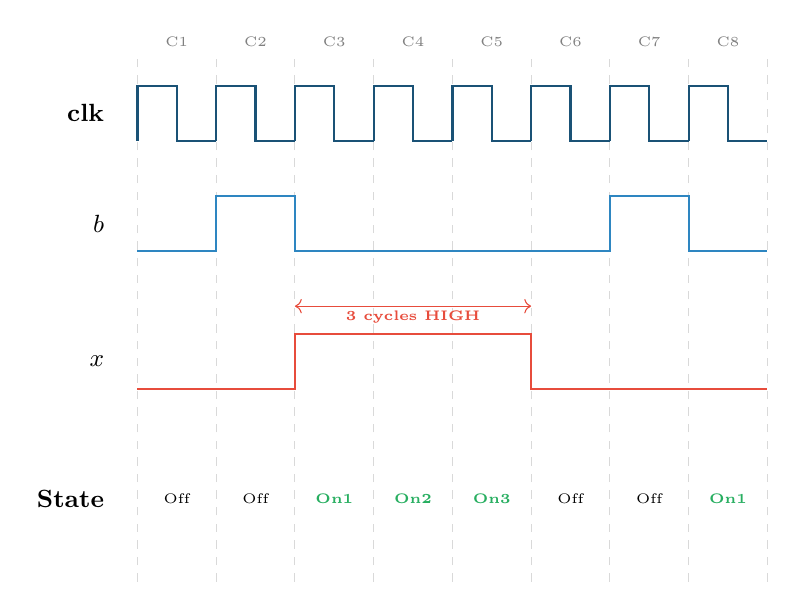
\begin{tikzpicture}[xscale=1.0, yscale=0.7]
  % Grid
  \foreach \x in {0,1,...,8} {
    \draw[gray!30, dashed] (\x, -8.5) -- (\x, 1);
  }
  
  % Clock signal
  \node[left, font=\small\bfseries] at (-0.3, 0) {clk};
  \foreach \x in {0,1,...,7} {
    \draw[thick, primary] (\x, -0.5) -- (\x, 0.5) -- (\x+0.5, 0.5) -- (\x+0.5, -0.5) -- (\x+1, -0.5);
  }
  
  % Button b
  \node[left, font=\small\bfseries] at (-0.3, -2) {$b$};
  \draw[thick, accent] (0,-2.5) -- (1,-2.5) -- (1,-1.5) -- (2,-1.5) -- (2,-2.5) -- (6,-2.5) -- (6,-1.5) -- (7,-1.5) -- (7,-2.5) -- (8,-2.5);
  
  % Output x
  \node[left, font=\small\bfseries] at (-0.3, -4.5) {$x$};
  \draw[thick, highlight] (0,-5) -- (2,-5) -- (2,-4) -- (5,-4) -- (5,-5) -- (8,-5);
  \node[font=\tiny, highlight] at (3.5, -3.7) {\textbf{3 cycles HIGH}};
  \draw[highlight, <->] (2,-3.5) -- (5,-3.5);

  % State
  \node[left, font=\small\bfseries] at (-0.3, -7) {State};
  \node[font=\tiny] at (0.5, -7) {Off};
  \node[font=\tiny] at (1.5, -7) {Off};
  \node[font=\tiny, success] at (2.5, -7) {\textbf{On1}};
  \node[font=\tiny, success] at (3.5, -7) {\textbf{On2}};
  \node[font=\tiny, success] at (4.5, -7) {\textbf{On3}};
  \node[font=\tiny] at (5.5, -7) {Off};
  \node[font=\tiny] at (6.5, -7) {Off};
  \node[font=\tiny, success] at (7.5, -7) {\textbf{On1}};
  
  % Cycle labels
  \foreach \x [count=\i] in {0,1,...,7} {
    \node[font=\tiny, gray] at (\x+0.5, 1.3) {C\i};
  }
\end{tikzpicture}
\caption{Timing diagram for the laser timer}
\end{figure}

% ═══════════════════════════════════════════════════════
% SECTION 5: 5-STEP CONTROLLER DESIGN PROCESS
% ═══════════════════════════════════════════════════════
\section{The 5-Step Controller Design Process}

This is the \textbf{core methodology} for converting any FSM into a working digital circuit.

\subsection{Overview of Steps}

\begin{table}[H]
\centering
\renewcommand{\arraystretch}{1.5}
\begin{tabular}{@{} >{\bfseries}c >{\bfseries}l p{8.5cm} @{}}
  \toprule
  Step & Name & What You Do \\
  \midrule
  1 & Capture the FSM & Draw the FSM state diagram describing desired behavior \\
  \addlinespace
  2A & Set Up Architecture & Use state register (D flip-flops) + combinational logic block \\
  \addlinespace
  2B & Encode the States & Assign a unique binary number to each state \\
  \addlinespace
  2C & Fill the Truth Table & Translate all FSM transitions into truth table rows \\
  \addlinespace
  2D & Implement Comb. Logic & Derive Boolean equations from truth table, build gates \\
  \bottomrule
\end{tabular}
\caption{The 5-step controller design process (Table 3.2 from textbook)}
\label{tab:5step}
\end{table}

\subsection{The Standard Architecture}

Every FSM controller uses the \textbf{same} architecture:

\begin{figure}[H]
\centering
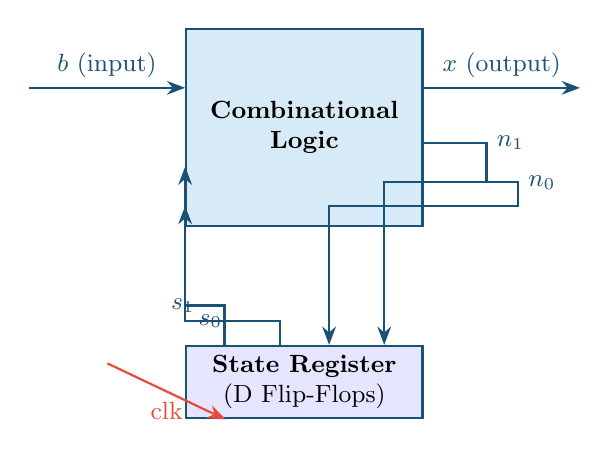
\begin{tikzpicture}[node distance=1.5cm]
  % Blocks
  \node[block, minimum height=2.5cm, minimum width=3cm] (comb) {\textbf{Combinational}\\\textbf{Logic}};
  \node[register, below=1.5cm of comb, minimum width=3cm] (reg) {\textbf{State Register}\\(D Flip-Flops)};
  
  % Input
  \draw[io] (-3.5, 0.5) -- node[above, font=\small]{$b$ (input)} (comb.west |- 0,0.5);
  
  % Output x
  \draw[io] (comb.east |- 0,0.5) -- node[above, font=\small]{$x$ (output)} (3.5, 0.5);
  
  % Next state outputs
  \draw[io] (comb.east |- 0,-0.2) -- ++(0.8,0) node[right, font=\small]{$n_1$} -- ++(0,-0.5) -| ($(reg.north east) + (-0.5, 0)$);
  \draw[io] (comb.east |- 0,-0.7) -- ++(1.2,0) node[right, font=\small]{$n_0$} -- ++(0,-0.3) -| ($(reg.north east) + (-1.2, 0)$);
  
  % Current state feedback
  \draw[io] ($(reg.north west) + (0.5, 0)$) -- ++(0, 0.5) -| ($(comb.west) + (0, -0.5)$) node[near start, left, font=\small]{$s_1$};
  \draw[io] ($(reg.north west) + (1.2, 0)$) -- ++(0, 0.3) -| ($(comb.west) + (0, -1.0)$) node[near start, left, font=\small]{$s_0$};
  
  % Clock
  \draw[clk] (-2.5, -3) -- node[below, font=\small\color{highlight}]{clk} (reg.south -| -1,0);
  
\end{tikzpicture}
\caption{Standard FSM controller architecture}
\label{fig:architecture}
\end{figure}

\begin{keypoint}[How It Works --- Every Clock Cycle]
  \begin{enumerate}
    \item On each \textbf{rising clock edge}, the state register captures $n_1, n_0$ and stores them as $s_1, s_0$
    \item The combinational logic reads \textbf{current state} ($s_1, s_0$) and \textbf{input} ($b$)
    \item It computes the \textbf{output} ($x$) and the \textbf{next state} ($n_1, n_0$)
    \item Repeat!
  \end{enumerate}
\end{keypoint}

% ═══════════════════════════════════════════════════════
% SECTION 6: STEP-BY-STEP CONVERSION
% ═══════════════════════════════════════════════════════
\section{Step-by-Step: Converting Laser Timer FSM to Circuit}

\subsection{Step 2B: Encode the States}

\begin{table}[H]
\centering
\renewcommand{\arraystretch}{1.3}
\begin{tabular}{@{} >{\bfseries}c c c c @{}}
  \toprule
  State & $s_1$ & $s_0$ & Binary Encoding \\
  \midrule
  Off & 0 & 0 & \texttt{00} \\
  On1 & 0 & 1 & \texttt{01} \\
  On2 & 1 & 0 & \texttt{10} \\
  On3 & 1 & 1 & \texttt{11} \\
  \bottomrule
\end{tabular}
\caption{State encoding for laser timer}
\end{table}

\subsection{Step 2C: Fill the Truth Table}

For each combination of current state ($s_1, s_0$) and input ($b$), determine output ($x$) and next state ($n_1, n_0$):

\begin{table}[H]
\centering
\renewcommand{\arraystretch}{1.3}
\begin{tabular}{@{} >{\bfseries}c | c c c | c c c | l @{}}
  \toprule
  \multirow{2}{*}{State} & \multicolumn{3}{c|}{\textbf{Inputs}} & \multicolumn{3}{c|}{\textbf{Outputs}} & \multirow{2}{*}{\textbf{Explanation}} \\
  & $s_1$ & $s_0$ & $b$ & $x$ & $n_1$ & $n_0$ & \\
  \midrule
  \multirow{2}{*}{Off} 
    & 0 & 0 & 0 & 0 & 0 & 0 & $b{=}0$: stay in Off \\
    & 0 & 0 & 1 & 0 & 0 & 1 & $b{=}1$: go to On1 \\
  \midrule
  \multirow{2}{*}{On1}
    & 0 & 1 & 0 & 1 & 1 & 0 & always $\to$ On2 \\
    & 0 & 1 & 1 & 1 & 1 & 0 & always $\to$ On2 \\
  \midrule
  \multirow{2}{*}{On2}
    & 1 & 0 & 0 & 1 & 1 & 1 & always $\to$ On3 \\
    & 1 & 0 & 1 & 1 & 1 & 1 & always $\to$ On3 \\
  \midrule
  \multirow{2}{*}{On3}
    & 1 & 1 & 0 & 1 & 0 & 0 & always $\to$ Off \\
    & 1 & 1 & 1 & 1 & 0 & 0 & always $\to$ Off \\
  \bottomrule
\end{tabular}
\caption{Complete truth table for the laser timer controller}
\label{tab:truth-laser}
\end{table}

\begin{tip}[How to Read Each Row]
  \textbf{Row 2:} Current state = Off ($s_1{=}0, s_0{=}0$), button pressed ($b{=}1$).\\
  From FSM: Off $\to$ On1 when $b{=}1$. On1's encoding is \texttt{01}, so $n_1{=}0, n_0{=}1$.\\
  Off's output: $x{=}0$.
  
  \vspace{4pt}
  \textbf{Row 3:} Current state = On1 ($s_1{=}0, s_0{=}1$), $b{=}0$.\\
  From FSM: On1 $\to$ On2 (unconditional). On2's encoding is \texttt{10}, so $n_1{=}1, n_0{=}0$.\\
  On1's output: $x{=}1$.
\end{tip}

\subsection{Step 2D: Derive Boolean Equations}

\subsubsection*{Output $x$:}

From the truth table, $x = 1$ in rows 3--8 (all states except Off):
\begin{align*}
  x &= \overline{s_1} \cdot s_0 + s_1 \cdot \overline{s_0} + s_1 \cdot s_0 \\
  x &= s_0 + s_1
\end{align*}

\begin{equation}
  \boxed{x = s_1 + s_0}
\end{equation}

\textit{Output is 1 whenever we're NOT in the Off state (00).}

\subsubsection*{Next State $n_1$:}

$n_1 = 1$ when state is On1 ($s_1{=}0, s_0{=}1$) or On2 ($s_1{=}1, s_0{=}0$), regardless of $b$:
\begin{align*}
  n_1 &= \overline{s_1} \cdot s_0 + s_1 \cdot \overline{s_0}
\end{align*}

\begin{equation}
  \boxed{n_1 = s_1 \oplus s_0}
\end{equation}

\textit{This is the XOR of the two state bits.}

\subsubsection*{Next State $n_0$:}

$n_0 = 1$ when: Off with $b{=}1$, or On2 (regardless of $b$):
\begin{align*}
  n_0 &= \overline{s_1} \cdot \overline{s_0} \cdot b + s_1 \cdot \overline{s_0} \cdot \overline{b} + s_1 \cdot \overline{s_0} \cdot b \\
  n_0 &= \overline{s_1} \cdot \overline{s_0} \cdot b + s_1 \cdot \overline{s_0} \\
  n_0 &= \overline{s_0} \cdot (\overline{s_1} \cdot b + s_1) \\
  n_0 &= \overline{s_0} \cdot (s_1 + b) \quad \text{(using } A + \overline{A} \cdot B = A + B \text{)}
\end{align*}

\begin{equation}
  \boxed{n_0 = \overline{s_0} \cdot (s_1 + b)}
\end{equation}

\subsection{K-Map Derivation (Karnaugh Maps)}

Now we use \textbf{Karnaugh Maps} to systematically derive minimized Boolean equations from the truth table. For a D flip-flop, the key rule is:

\begin{important}[D Flip-Flop Rule]
  For D flip-flops, the \textbf{D input} equals the \textbf{next state}:\\[4pt]
  $D_1 = n_1$ \qquad (what gets loaded into flip-flop 1 at next clock edge)\\
  $D_0 = n_0$ \qquad (what gets loaded into flip-flop 0 at next clock edge)\\[4pt]
  So our job is to find the equations for $D_1$ and $D_0$ from the truth table.
\end{important}

\subsubsection*{K-Map for Output $x$}

\begin{figure}[H]
\centering
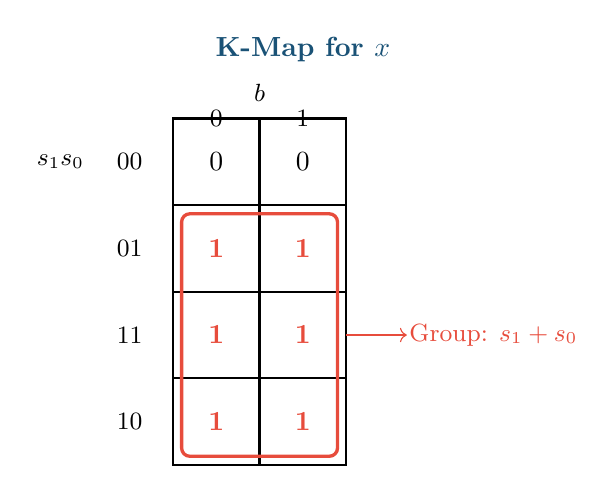
\begin{tikzpicture}[scale=1.1]
  % Title
  \node[font=\bfseries\color{primary}] at (2, 3.8) {K-Map for $x$};
  
  % Headers
  \node[font=\small] at (-0.8, 2.5) {$s_1 s_0$};
  \node[font=\small] at (1.5, 3.3) {$b$};
  \node[font=\small] at (1, 3) {0};
  \node[font=\small] at (2, 3) {1};
  
  % Row labels
  \node[font=\small] at (0, 2.5) {00};
  \node[font=\small] at (0, 1.5) {01};
  \node[font=\small] at (0, 0.5) {11};
  \node[font=\small] at (0, -0.5) {10};
  
  % Grid
  \draw[thick] (0.5, -1) -- (0.5, 3) -- (2.5, 3) -- (2.5, -1) -- cycle;
  \draw[thick] (1.5, -1) -- (1.5, 3);
  \draw[thick] (0.5, 2) -- (2.5, 2);
  \draw[thick] (0.5, 1) -- (2.5, 1);
  \draw[thick] (0.5, 0) -- (2.5, 0);
  
  % Values
  \node at (1, 2.5) {0};
  \node at (2, 2.5) {0};
  \node[font=\bfseries, color=highlight] at (1, 1.5) {1};
  \node[font=\bfseries, color=highlight] at (2, 1.5) {1};
  \node[font=\bfseries, color=highlight] at (1, 0.5) {1};
  \node[font=\bfseries, color=highlight] at (2, 0.5) {1};
  \node[font=\bfseries, color=highlight] at (1, -0.5) {1};
  \node[font=\bfseries, color=highlight] at (2, -0.5) {1};
  
  % Grouping - group all 1s (rows 01, 11, 10)
  \draw[very thick, highlight, rounded corners=3pt] (0.6, -0.9) rectangle (2.4, 1.9);
  \node[font=\small, highlight] at (4.2, 0.5) {Group: $s_1 + s_0$};
  \draw[highlight, ->] (2.5, 0.5) -- (3.2, 0.5);
\end{tikzpicture}
\caption{K-Map for output $x$ --- all non-Off states give $x=1$}
\end{figure}

\begin{equation}
  \boxed{x = s_1 + s_0}
\end{equation}

\textit{Meaning: Output $x=1$ whenever the FSM is NOT in state Off ($s_1 s_0 = 00$).}

\subsubsection*{K-Map for $D_1$ (= $n_1$, D input of flip-flop 1)}

\begin{figure}[H]
\centering
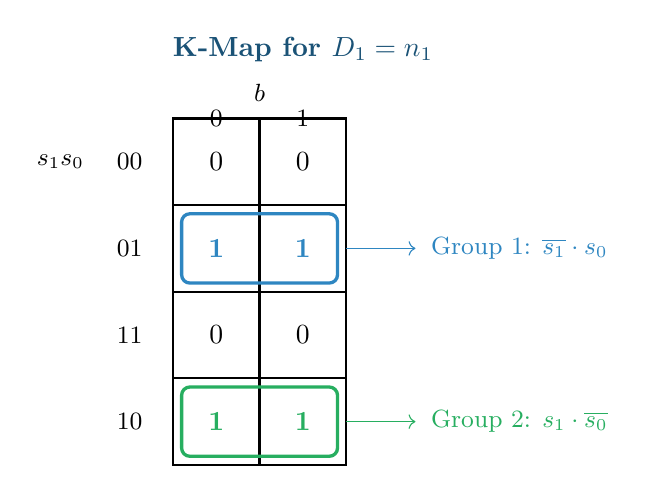
\begin{tikzpicture}[scale=1.1]
  % Title
  \node[font=\bfseries\color{primary}] at (2, 3.8) {K-Map for $D_1 = n_1$};
  
  % Headers
  \node[font=\small] at (-0.8, 2.5) {$s_1 s_0$};
  \node[font=\small] at (1.5, 3.3) {$b$};
  \node[font=\small] at (1, 3) {0};
  \node[font=\small] at (2, 3) {1};
  
  % Row labels
  \node[font=\small] at (0, 2.5) {00};
  \node[font=\small] at (0, 1.5) {01};
  \node[font=\small] at (0, 0.5) {11};
  \node[font=\small] at (0, -0.5) {10};
  
  % Grid
  \draw[thick] (0.5, -1) -- (0.5, 3) -- (2.5, 3) -- (2.5, -1) -- cycle;
  \draw[thick] (1.5, -1) -- (1.5, 3);
  \draw[thick] (0.5, 2) -- (2.5, 2);
  \draw[thick] (0.5, 1) -- (2.5, 1);
  \draw[thick] (0.5, 0) -- (2.5, 0);
  
  % Values
  \node at (1, 2.5) {0};
  \node at (2, 2.5) {0};
  \node[font=\bfseries, color=accent] at (1, 1.5) {1};
  \node[font=\bfseries, color=accent] at (2, 1.5) {1};
  \node at (1, 0.5) {0};
  \node at (2, 0.5) {0};
  \node[font=\bfseries, color=success] at (1, -0.5) {1};
  \node[font=\bfseries, color=success] at (2, -0.5) {1};
  
  % Group 1: s0=1, s1=0 row (01)
  \draw[very thick, accent, rounded corners=3pt] (0.6, 1.1) rectangle (2.4, 1.9);
  \node[font=\small, accent] at (4.5, 1.5) {Group 1: $\overline{s_1} \cdot s_0$};
  \draw[accent, ->] (2.5, 1.5) -- (3.3, 1.5);
  
  % Group 2: s1=1, s0=0 row (10)
  \draw[very thick, success, rounded corners=3pt] (0.6, -0.9) rectangle (2.4, -0.1);
  \node[font=\small, success] at (4.5, -0.5) {Group 2: $s_1 \cdot \overline{s_0}$};
  \draw[success, ->] (2.5, -0.5) -- (3.3, -0.5);
\end{tikzpicture}
\caption{K-Map for $D_1$ --- two separate groups that cannot be combined}
\end{figure}

The two groups are \textbf{not adjacent} in the K-Map, so they cannot be combined further:

\begin{align}
  D_1 &= \overline{s_1} \cdot s_0 + s_1 \cdot \overline{s_0}
\end{align}

\begin{equation}
  \boxed{D_1 = s_1 \oplus s_0 \qquad \text{(XOR gate)}}
\end{equation}

\begin{tip}[Why XOR?]
  $\overline{A} \cdot B + A \cdot \overline{B}$ is the \textbf{definition} of XOR ($A \oplus B$).\\
  So $D_1$ needs just \textbf{one XOR gate}!
\end{tip}

\subsubsection*{K-Map for $D_0$ (= $n_0$, D input of flip-flop 0)}

\begin{figure}[H]
\centering
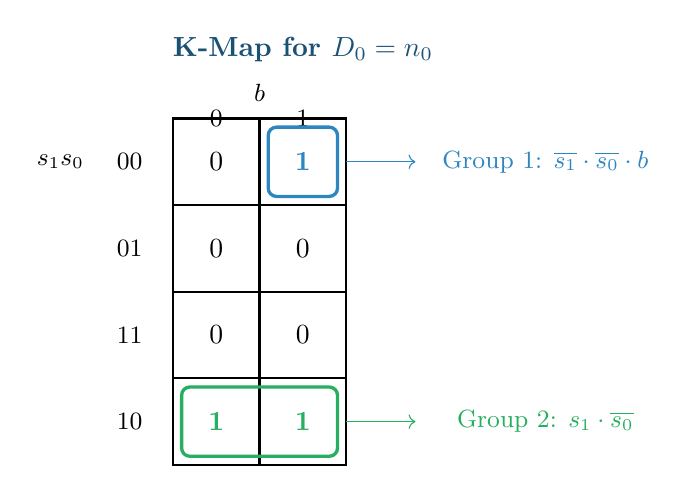
\begin{tikzpicture}[scale=1.1]
  % Title
  \node[font=\bfseries\color{primary}] at (2, 3.8) {K-Map for $D_0 = n_0$};
  
  % Headers
  \node[font=\small] at (-0.8, 2.5) {$s_1 s_0$};
  \node[font=\small] at (1.5, 3.3) {$b$};
  \node[font=\small] at (1, 3) {0};
  \node[font=\small] at (2, 3) {1};
  
  % Row labels
  \node[font=\small] at (0, 2.5) {00};
  \node[font=\small] at (0, 1.5) {01};
  \node[font=\small] at (0, 0.5) {11};
  \node[font=\small] at (0, -0.5) {10};
  
  % Grid
  \draw[thick] (0.5, -1) -- (0.5, 3) -- (2.5, 3) -- (2.5, -1) -- cycle;
  \draw[thick] (1.5, -1) -- (1.5, 3);
  \draw[thick] (0.5, 2) -- (2.5, 2);
  \draw[thick] (0.5, 1) -- (2.5, 1);
  \draw[thick] (0.5, 0) -- (2.5, 0);
  
  % Values
  \node at (1, 2.5) {0};
  \node[font=\bfseries, color=accent] at (2, 2.5) {1};
  \node at (1, 1.5) {0};
  \node at (2, 1.5) {0};
  \node at (1, 0.5) {0};
  \node at (2, 0.5) {0};
  \node[font=\bfseries, color=success] at (1, -0.5) {1};
  \node[font=\bfseries, color=success] at (2, -0.5) {1};
  
  % Group 1: s1=0, s0=0, b=1 (single cell)
  \draw[very thick, accent, rounded corners=3pt] (1.6, 2.1) rectangle (2.4, 2.9);
  \node[font=\small, accent] at (4.8, 2.5) {Group 1: $\overline{s_1} \cdot \overline{s_0} \cdot b$};
  \draw[accent, ->] (2.5, 2.5) -- (3.3, 2.5);
  
  % Group 2: s1=1, s0=0 row (10) - both b=0 and b=1
  \draw[very thick, success, rounded corners=3pt] (0.6, -0.9) rectangle (2.4, -0.1);
  \node[font=\small, success] at (4.8, -0.5) {Group 2: $s_1 \cdot \overline{s_0}$};
  \draw[success, ->] (2.5, -0.5) -- (3.3, -0.5);
\end{tikzpicture}
\caption{K-Map for $D_0$ --- one pair and one single cell}
\end{figure}

From the K-Map:
\begin{align}
  D_0 &= \overline{s_1} \cdot \overline{s_0} \cdot b \ + \ s_1 \cdot \overline{s_0} \\[6pt]
  D_0 &= \overline{s_0} \cdot (\overline{s_1} \cdot b + s_1) \\[6pt]
  D_0 &= \overline{s_0} \cdot (s_1 + b) \quad \text{(using Boolean identity: } A + \overline{A}B = A + B\text{)}
\end{align}

\begin{equation}
  \boxed{D_0 = \overline{s_0} \cdot (s_1 + b)}
\end{equation}

\begin{tip}[Simplification Step-by-Step]
  \begin{enumerate}
    \item Start: $\overline{s_1} \cdot \overline{s_0} \cdot b + s_1 \cdot \overline{s_0}$
    \item Factor out $\overline{s_0}$: \ $\overline{s_0} \cdot (\overline{s_1} \cdot b + s_1)$
    \item Apply $A + \overline{A}B = A+B$ where $A = s_1$, $B = b$: \ $\overline{s_0} \cdot (s_1 + b)$
  \end{enumerate}
  This requires: \textbf{1 NOT gate + 1 OR gate + 1 AND gate}
\end{tip}

% ─────────────────────────────────────────────────────
\subsection{Summary of All D Flip-Flop Input Equations}

\begin{keypoint}[Complete Design Equations]
  These are the \textbf{final equations} needed to build the hardware:\\[8pt]
  \renewcommand{\arraystretch}{1.8}
  \begin{tabular}{@{} >{\bfseries}l l l @{}}
    Signal & Equation & Hardware Needed \\
    \hline
    Output: & $x = s_1 + s_0$ & 1 OR gate \\
    FF1 input: & $D_1 = s_1 \oplus s_0$ & 1 XOR gate \\
    FF0 input: & $D_0 = \overline{s_0} \cdot (s_1 + b)$ & 1 NOT + 1 OR + 1 AND gate \\
  \end{tabular}
\end{keypoint}

% ─────────────────────────────────────────────────────
\subsection{Complete Hardware Circuit with D Flip-Flops}

Below is the \textbf{complete circuit} showing exactly how to wire two D flip-flops with the combinational logic gates:

\begin{figure}[H]
\centering
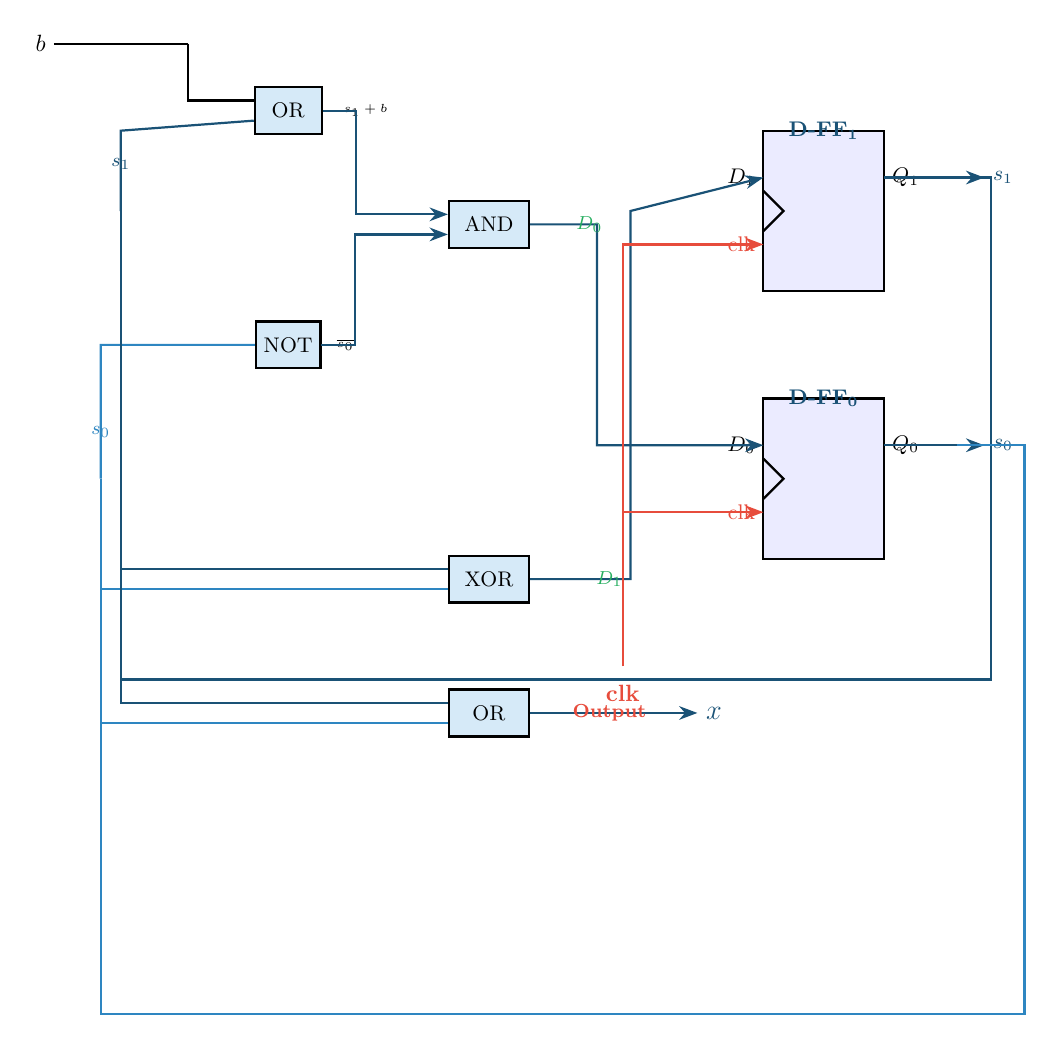
\begin{tikzpicture}[scale=0.85, transform shape,
  dff/.style={draw, thick, fill=blue!8, minimum width=1.8cm, minimum height=2.4cm, align=center},
  gate/.style={draw, thick, fill=statebg, minimum width=1cm, minimum height=0.7cm, font=\small},
  sig/.style={-Stealth, thick, primary},
  clksig/.style={-Stealth, thick, highlight}]

  % ====== D FLIP-FLOPS ======
  
  % FF1 (stores s1)
  \node[dff] (ff1) at (11, -1) {};
  \node[font=\bfseries\small, primary] at (11, 0.2) {D-FF\textsubscript{1}};
  \node[font=\small, left] at (10.1, -0.5) {$D_1$};
  \node[font=\small, right] at (11.9, -0.5) {$Q_1$};
  \node[font=\small, left] at (10.1, -1.5) {\textcolor{highlight}{clk}};
  \draw[thick] (10.1, -1.3) -- (10.4, -1.0) -- (10.1, -0.7); % clock triangle
  
  % FF0 (stores s0)
  \node[dff] (ff0) at (11, -5) {};
  \node[font=\bfseries\small, primary] at (11, -3.8) {D-FF\textsubscript{0}};
  \node[font=\small, left] at (10.1, -4.5) {$D_0$};
  \node[font=\small, right] at (11.9, -4.5) {$Q_0$};
  \node[font=\small, left] at (10.1, -5.5) {\textcolor{highlight}{clk}};
  \draw[thick] (10.1, -5.3) -- (10.4, -5.0) -- (10.1, -4.7); % clock triangle
  
  % ====== OUTPUTS FROM FF ======
  
  % s1 output from FF1
  \draw[sig] (11.9, -0.5) -- ++(1.5, 0) node[right, font=\small\bfseries]{$s_1$};
  \coordinate (s1out) at (13.0, -0.5);
  
  % s0 output from FF0
  \draw[sig] (11.9, -4.5) -- ++(1.5, 0) node[right, font=\small\bfseries]{$s_0$};
  \coordinate (s0out) at (13.0, -4.5);
  
  % ====== FEEDBACK LINES ======
  
  % s1 feedback (goes left and down)
  \draw[thick, primary] (13.0, -0.5) -- ++(0.5, 0) -- ++(0, -7.5) -- ++(-13, 0) -- ++(0, 7);
  \coordinate (s1fb) at (0.5, -1);
  
  % s0 feedback
  \draw[thick, accent] (13.0, -4.5) -- ++(1.0, 0) -- ++(0, -8.5) -- ++(-13.8, 0) -- ++(0, 8);
  \coordinate (s0fb) at (0.2, -5);
  
  % ====== INPUT ======
  \node[left, font=\bfseries] at (-0.5, 1.5) {$b$};
  \draw[thick] (-0.5, 1.5) -- (1.5, 1.5);
  
  % ====== LABELS for feedback ======
  \node[font=\footnotesize, primary] at (0.5, -0.3) {$s_1$};
  \node[font=\footnotesize, accent] at (0.2, -4.3) {$s_0$};
  
  % ====== GATE: OR for (s1 + b) ======
  \node[gate] (or1) at (3, 0.5) {OR};
  \draw[thick] (1.5, 1.5) |- ($(or1.west) + (0, 0.15)$);
  \draw[thick, primary] (0.5, -1) -- (0.5, 0.2) -- ($(or1.west) + (0, -0.15)$);
  \node[font=\tiny, right] at (3.7, 0.5) {$s_1 + b$};
  
  % ====== GATE: NOT for s0' ======
  \node[gate, minimum width=0.8cm] (not1) at (3, -3) {NOT};
  \draw[thick, accent] (0.2, -5) -- (0.2, -3) -- (not1.west);
  \node[font=\tiny, right] at (3.6, -3) {$\overline{s_0}$};
  
  % ====== GATE: AND for D0 = s0' * (s1 + b) ======
  \node[gate, minimum width=1.2cm] (and1) at (6, -1.2) {AND};
  \draw[sig] (or1.east) -- ++(0.5, 0) |- ($(and1.west) + (0, 0.15)$);
  \draw[sig] (not1.east) -- ++(0.5, 0) |- ($(and1.west) + (0, -0.15)$);
  
  % Connect AND output to D0
  \draw[sig] (and1.east) -- ++(1, 0) -- ++(0, -3.3) -- (10.1, -4.5);
  \node[font=\footnotesize\bfseries, success] at (7.5, -1.2) {$D_0$};
  
  % ====== GATE: XOR for D1 = s1 XOR s0 ======
  \node[gate, minimum width=1.2cm] (xor1) at (6, -6.5) {XOR};
  \draw[thick, primary] (0.5, -1) -- (0.5, -6.35) -- (xor1.west |- 0,-6.35);
  \draw[thick, accent] (0.2, -5) -- (0.2, -6.65) -- (xor1.west |- 0,-6.65);
  
  % Connect XOR output to D1
  \draw[sig] (xor1.east) -- ++(1.5, 0) -- ++(0, 5.5) -- (10.1, -0.5);
  \node[font=\footnotesize\bfseries, success] at (7.8, -6.5) {$D_1$};
  
  % ====== GATE: OR for x = s1 + s0 ======
  \node[gate, minimum width=1.2cm] (or2) at (6, -8.5) {OR};
  \draw[thick, primary] (0.5, -1) -- (0.5, -8.35) -- (or2.west |- 0,-8.35);
  \draw[thick, accent] (0.2, -5) -- (0.2, -8.65) -- (or2.west |- 0,-8.65);
  \draw[sig] (or2.east) -- ++(2.5, 0) node[right, font=\bfseries\large]{$x$};
  \node[font=\footnotesize\bfseries, highlight] at (7.8, -8.5) {Output};
  
  % ====== CLOCK ======
  \draw[clksig] (8, -7.8) -- (8, -5.5) -- (10.1, -5.5);
  \draw[clksig] (8, -7.8) -- (8, -1.5) -- (10.1, -1.5);
  \node[font=\bfseries\color{highlight}] at (8, -8.2) {clk};
  
\end{tikzpicture}
\caption{Complete hardware circuit for the three-cycles-high laser timer using D flip-flops}
\label{fig:complete-circuit}
\end{figure}

\begin{keypoint}[Circuit Component Count]
  \renewcommand{\arraystretch}{1.4}
  \begin{tabular}{@{} l c l @{}}
    \textbf{Component} & \textbf{Qty} & \textbf{Purpose} \\
    \hline
    D Flip-Flop & 2 & Store $s_1$ (FF\textsubscript{1}) and $s_0$ (FF\textsubscript{0}) \\
    OR gate & 2 & One for $x = s_1 + s_0$, one for $s_1 + b$ in $D_0$ \\
    XOR gate & 1 & For $D_1 = s_1 \oplus s_0$ \\
    AND gate & 1 & For $D_0 = \overline{s_0} \cdot (s_1 + b)$ \\
    NOT gate & 1 & For $\overline{s_0}$ in $D_0$ \\
    \hline
    \textbf{Total} & \textbf{7} & \textbf{2 FFs + 5 gates}
  \end{tabular}
\end{keypoint}

% ─────────────────────────────────────────────────────
\subsection{Verification: Trace Through the Circuit}

Let's verify the circuit by tracing it through each state:

\begin{table}[H]
\centering
\renewcommand{\arraystretch}{1.4}
\begin{tabular}{@{} >{\bfseries}c | c c | c | c c c | c c | l @{}}
  \toprule
  \multirow{2}{*}{State} & \multicolumn{2}{c|}{Current} & \multirow{2}{*}{$b$} & \multicolumn{3}{c|}{Gate Outputs} & \multicolumn{2}{c|}{Next Clk Edge} & \multirow{2}{*}{Correct?} \\
  & $s_1$ & $s_0$ & & $x$ & $D_1$ & $D_0$ & $s_1'$ & $s_0'$ & \\
  \midrule
  Off  & 0 & 0 & 0 & 0 & 0 & 0 & 0 & 0 & \textcolor{success}{\checkmark} Off \\
  Off  & 0 & 0 & 1 & 0 & 0 & 1 & 0 & 1 & \textcolor{success}{\checkmark} On1 \\
  On1  & 0 & 1 & -- & 1 & 1 & 0 & 1 & 0 & \textcolor{success}{\checkmark} On2 \\
  On2  & 1 & 0 & -- & 1 & 1 & 1 & 1 & 1 & \textcolor{success}{\checkmark} On3 \\
  On3  & 1 & 1 & -- & 1 & 0 & 0 & 0 & 0 & \textcolor{success}{\checkmark} Off \\
  \bottomrule
\end{tabular}
\caption{Circuit verification --- traces match the FSM exactly}
\end{table}

Let's verify one row \textbf{manually}:

\begin{tip}[{Manual Trace: State = On2 ($s_1{=}1, s_0{=}0$)}]
  \begin{enumerate}
    \item $x = s_1 + s_0 = 1 + 0 = 1$ \quad \textcolor{success}{\checkmark} (laser ON)
    \item $D_1 = s_1 \oplus s_0 = 1 \oplus 0 = 1$
    \item $D_0 = \overline{s_0} \cdot (s_1 + b) = \overline{0} \cdot (1 + b) = 1 \cdot 1 = 1$
    \item At next clock edge: $s_1 \leftarrow D_1 = 1$, \ $s_0 \leftarrow D_0 = 1$
    \item New state: $s_1 s_0 = 11 =$ On3 \quad \textcolor{success}{\checkmark}
  \end{enumerate}
\end{tip}

% ─────────────────────────────────────────────────────
\subsection{Hardware Connection Summary}

For breadboard or schematic implementation, here is the complete wiring list:

\begin{table}[H]
\centering
\renewcommand{\arraystretch}{1.4}
\begin{tabular}{@{} c l l l @{}}
  \toprule
  \textbf{\#} & \textbf{From} & \textbf{To} & \textbf{Signal} \\
  \midrule
  1 & Input $b$ & OR\textsubscript{1} pin A & External button \\
  2 & FF\textsubscript{1} $Q$ output & OR\textsubscript{1} pin B & Feedback $s_1$ \\
  3 & OR\textsubscript{1} output & AND pin A & $s_1 + b$ \\
  4 & FF\textsubscript{0} $Q$ output & NOT input & Feedback $s_0$ \\
  5 & NOT output & AND pin B & $\overline{s_0}$ \\
  6 & AND output & FF\textsubscript{0} $D$ input & $D_0 = \overline{s_0} \cdot (s_1 + b)$ \\
  7 & FF\textsubscript{1} $Q$ output & XOR pin A & Feedback $s_1$ \\
  8 & FF\textsubscript{0} $Q$ output & XOR pin B & Feedback $s_0$ \\
  9 & XOR output & FF\textsubscript{1} $D$ input & $D_1 = s_1 \oplus s_0$ \\
  10 & FF\textsubscript{1} $Q$ output & OR\textsubscript{2} pin A & $s_1$ \\
  11 & FF\textsubscript{0} $Q$ output & OR\textsubscript{2} pin B & $s_0$ \\
  12 & OR\textsubscript{2} output & Output $x$ & $x = s_1 + s_0$ (laser) \\
  13 & Clock oscillator & FF\textsubscript{1} clk \& FF\textsubscript{0} clk & System clock \\
  \bottomrule
\end{tabular}
\caption{Complete wiring list for hardware implementation}
\label{tab:wiring}
\end{table}

% ═══════════════════════════════════════════════════════
% SECTION 7: CALL/CANCEL LIGHT CONTROLLER
% ═══════════════════════════════════════════════════════
\section{Example 3 --- Call/Cancel Light Controller}

\subsection{Problem}
A hospital call light system: pressing \textbf{Call} turns the light ON; pressing \textbf{Cncl} turns it OFF. If both pressed simultaneously, the light \textbf{stays in its current state}.

\textbf{Inputs:} Call, Cncl \quad \textbf{Output:} $L$ (1 = light ON)

\subsection{FSM State Diagram}

\begin{figure}[H]
\centering
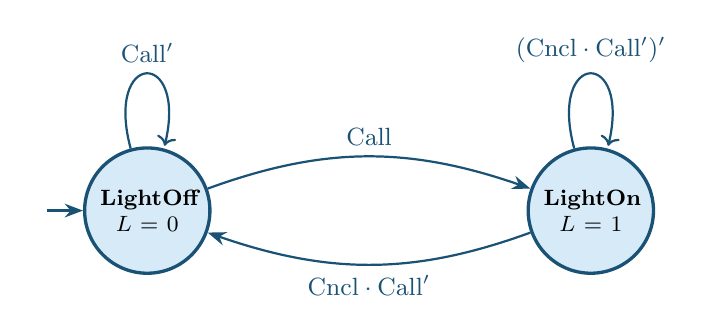
\begin{tikzpicture}[node distance=4cm]
  \node[fsm state, initial] (off) {\textbf{LightOff} \\ $L=0$};
  \node[fsm state, right=of off] (on) {\textbf{LightOn} \\ $L=1$};
  
  \draw[fsm arrow] (off) edge[loop above] node[above, align=center]{\small $\text{Call}'$} (off);
  \draw[fsm arrow] (off) to[bend left=20] node[above]{\small Call} (on);
  \draw[fsm arrow] (on) to[bend left=20] node[below, align=center]{\small $\text{Cncl} \cdot \text{Call}'$} (off);
  \draw[fsm arrow] (on) edge[loop above] node[above, align=center]{\small $(\text{Cncl} \cdot \text{Call}')'$} (on);
\end{tikzpicture}
\caption{FSM for hospital call/cancel light controller}
\end{figure}

\subsection{State Encoding \& Truth Table}

2 states $\Rightarrow$ 1 flip-flop: \ LightOff $= 0$, \ LightOn $= 1$

\begin{table}[H]
\centering
\renewcommand{\arraystretch}{1.3}
\begin{tabular}{@{} c c c | c c | l @{}}
  \toprule
  $s_0$ & Call & Cncl & $L$ & $n_0$ & Explanation \\
  \midrule
  0 & 0 & 0 & 0 & 0 & No call $\to$ stay off \\
  0 & 0 & 1 & 0 & 0 & Cancel while off $\to$ stay off \\
  0 & 1 & 0 & 0 & 1 & Call pressed $\to$ turn on \\
  0 & 1 & 1 & 0 & 1 & Call overrides $\to$ turn on \\
  \midrule
  1 & 0 & 0 & 1 & 1 & No input $\to$ stay on \\
  1 & 0 & 1 & 1 & 0 & Cancel $\to$ turn off \\
  1 & 1 & 0 & 1 & 1 & Call while on $\to$ stay on \\
  1 & 1 & 1 & 1 & 1 & Both pressed $\to$ stay on \\
  \bottomrule
\end{tabular}
\caption{Truth table for the call/cancel light controller}
\end{table}

\subsection{D Flip-Flop Equation \& Hardware Circuit}

Since there are only \textbf{2 states}, we need \textbf{1 D flip-flop}:

\begin{align}
  L  &= s_0 \quad \text{(output directly from FF)} \\[6pt]
  n_0 &= \overline{s_0} \cdot \text{Call} + s_0 \cdot \overline{\text{Cncl}} + s_0 \cdot \text{Call}
\end{align}

Simplifying using $s_0 \cdot \overline{\text{Cncl}} + s_0 \cdot \text{Call} = s_0 \cdot (\overline{\text{Cncl}} + \text{Call})$, and then $\overline{s_0} \cdot \text{Call} + s_0 \cdot \text{Call} = \text{Call}$:

\begin{equation}
  \boxed{D_0 = n_0 = \text{Call} + s_0 \cdot \overline{\text{Cncl}}}
\end{equation}

\begin{figure}[H]
\centering
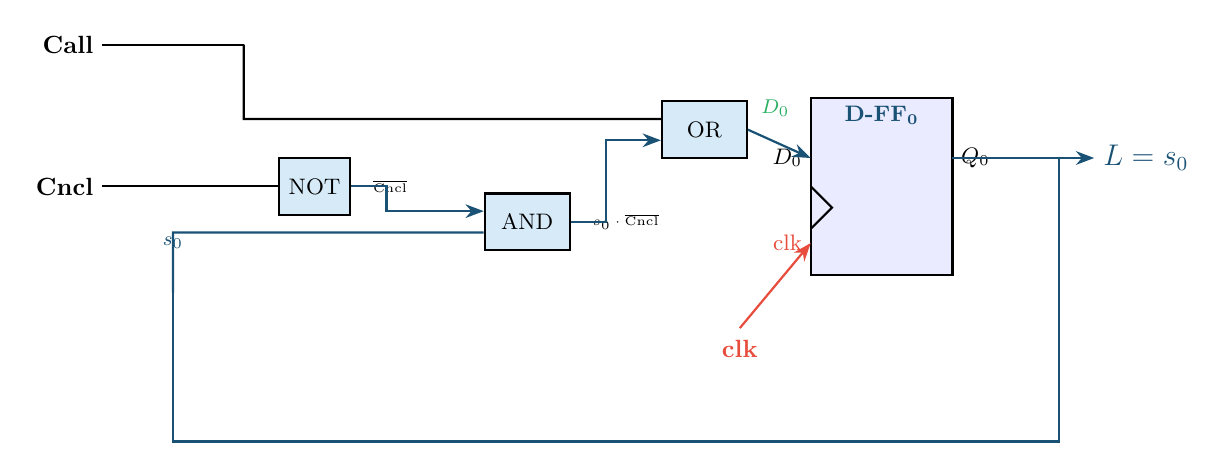
\begin{tikzpicture}[scale=0.9, transform shape,
  dff/.style={draw, thick, fill=blue!8, minimum width=2cm, minimum height=2.5cm, align=center},
  gate/.style={draw, thick, fill=statebg, minimum width=1.2cm, minimum height=0.8cm, font=\small},
  sig/.style={-Stealth, thick, primary},
  clksig/.style={-Stealth, thick, highlight}]
  
  % D Flip-Flop
  \node[dff] (ff) at (10, 0) {};
  \node[font=\bfseries\small, primary] at (10, 1.0) {D-FF\textsubscript{0}};
  \node[font=\small, left] at (9, 0.4) {$D_0$};
  \node[font=\small, right] at (11, 0.4) {$Q_0$};
  \node[font=\small, left] at (9, -0.8) {\textcolor{highlight}{clk}};
  \draw[thick] (9, -0.6) -- (9.3, -0.3) -- (9, 0); % clock triangle
  
  % Output from FF
  \draw[sig] (11, 0.4) -- ++(2, 0) node[right, font=\bfseries\large]{$L = s_0$};
  
  % Feedback s0
  \draw[thick, primary] (12.5, 0.4) -- ++(0, -4) -- ++(-12.5, 0) -- ++(0, 2.5);
  \node[font=\footnotesize, primary] at (0, -0.8) {$s_0$};
  
  % Inputs
  \node[left, font=\bfseries] at (-1, 2) {Call};
  \node[left, font=\bfseries] at (-1, 0) {Cncl};
  \draw[thick] (-1, 2) -- (1, 2);
  \draw[thick] (-1, 0) -- (0.5, 0);
  
  % NOT gate for Cncl'
  \node[gate, minimum width=1cm] (not1) at (2, 0) {NOT};
  \draw[thick] (0.5, 0) -- (not1.west);
  \node[font=\tiny, right] at (2.7, 0) {$\overline{\text{Cncl}}$};
  
  % AND gate for s0 * Cncl'
  \node[gate] (and1) at (5, -0.5) {AND};
  \draw[sig] (not1.east) -- ++(0.5, 0) |- ($(and1.west) + (0, 0.15)$);
  \draw[thick, primary] (0, -1.5) -- (0, -0.65) -- ($(and1.west) + (0, -0.15)$);
  \node[font=\tiny, right] at (5.8, -0.5) {$s_0 \cdot \overline{\text{Cncl}}$};
  
  % OR gate for D0 = Call + s0*Cncl'
  \node[gate] (or1) at (7.5, 0.8) {OR};
  \draw[thick] (1, 2) -- (1, 0.95) -- ($(or1.west) + (0, 0.15)$);
  \draw[sig] (and1.east) -- ++(0.5, 0) |- ($(or1.west) + (0, -0.15)$);
  
  % Connect OR to D input
  \draw[sig] (or1.east) -- (9, 0.4);
  \node[font=\footnotesize\bfseries, success] at (8.5, 1.1) {$D_0$};
  
  % Clock
  \draw[clksig] (8, -2) -- (9, -0.8);
  \node[font=\bfseries\color{highlight}] at (8, -2.3) {clk};
  
\end{tikzpicture}
\caption{Complete hardware circuit for call/cancel light using 1 D flip-flop}
\end{figure}

\begin{keypoint}[Component Count]
  \textbf{1 D-FF} + \textbf{1 NOT gate} + \textbf{1 AND gate} + \textbf{1 OR gate} = \textbf{4 components total}
\end{keypoint}

% ═══════════════════════════════════════════════════════
% SECTION 8: GLITCHING
% ═══════════════════════════════════════════════════════
\section{Output Glitching \& Solutions}

\subsection{What is Glitching?}

\begin{important}[Glitching Definition]
  \textbf{Glitching} = temporary incorrect output values that appear \textit{briefly} when the combinational logic computes new outputs after a state change, before stable values are reached.
\end{important}

\subsection{Why It Happens}

When the state register changes (e.g., from \texttt{01} to \texttt{10}), the bits don't switch at \textbf{exactly the same instant}:

\begin{figure}[H]
\centering
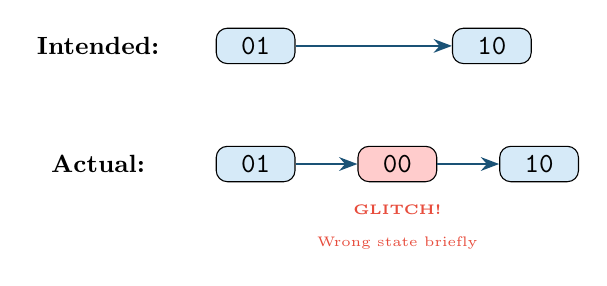
\begin{tikzpicture}
  % Intended
  \node[font=\small\bfseries] at (0, 1.5) {Intended:};
  \node[draw, rounded corners, fill=statebg, minimum width=1cm] (a1) at (2, 1.5) {\texttt{01}};
  \node[draw, rounded corners, fill=statebg, minimum width=1cm] (a2) at (5, 1.5) {\texttt{10}};
  \draw[fsm arrow] (a1) -- (a2);
  
  % Actual
  \node[font=\small\bfseries] at (0, 0) {Actual:};
  \node[draw, rounded corners, fill=statebg, minimum width=1cm] (b1) at (2, 0) {\texttt{01}};
  \node[draw, rounded corners, fill=red!20, minimum width=1cm] (b2) at (3.8, 0) {\texttt{00}};
  \node[draw, rounded corners, fill=statebg, minimum width=1cm] (b3) at (5.6, 0) {\texttt{10}};
  \draw[fsm arrow] (b1) -- (b2);
  \draw[fsm arrow] (b2) -- (b3);
  \node[font=\tiny\color{highlight}, below] at (3.8, -0.4) {\textbf{GLITCH!}};
  \node[font=\tiny\color{highlight}, below] at (3.8, -0.8) {Wrong state briefly};
\end{tikzpicture}
\caption{How glitching occurs during state transitions}
\end{figure}

\subsection{Solution 1: Registered Outputs}

Add a \textbf{D flip-flop} on each output to capture it only at the clock edge (when stable):

\begin{figure}[H]
\centering
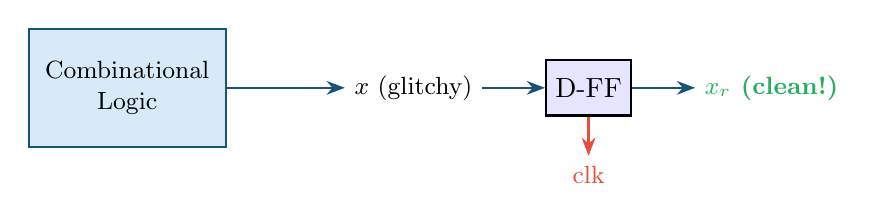
\begin{tikzpicture}[node distance=1.2cm]
  \node[block, minimum height=1.5cm] (comb) {Combinational\\Logic};
  \node[right=1.5cm of comb, font=\small] (xg) {$x$ (glitchy)};
  \node[draw, thick, fill=blue!10, right=0.8cm of xg, minimum width=1cm, minimum height=0.7cm] (dff) {D-FF};
  \node[right=0.8cm of dff, font=\small\bfseries\color{success}] (xr) {$x_r$ (clean!)};
  
  \draw[io] (comb.east) -- (xg);
  \draw[io] (xg) -- (dff.west);
  \draw[io] (dff.east) -- (xr);
  \draw[clk] (dff.south) -- ++(0,-0.5) node[below, font=\small\color{highlight}]{clk};
\end{tikzpicture}
\caption{Registered output solution --- adds 1 clock cycle delay but removes glitches}
\end{figure}

\textbf{Trade-off:} Output is delayed by \textbf{one clock cycle}.

\subsection{Solution 2: State Variables as Outputs}

Choose state encoding so the \textbf{state bits themselves} serve as outputs:

\begin{table}[H]
\centering
\renewcommand{\arraystretch}{1.3}
\begin{tabular}{@{} >{\bfseries}c c c c c @{}}
  \toprule
  State & $s_2$ & $s_1$ & $s_0$ & Output $x$ \\
  \midrule
  Off & 0 & 0 & 0 & $0 = s_0$ \\
  On1 & 0 & 1 & 1 & $1 = s_0$ \\
  On2 & 1 & 0 & 1 & $1 = s_0$ \\
  On3 & 1 & 1 & 1 & $1 = s_0$ \\
  \bottomrule
\end{tabular}
\caption{State-as-output encoding: $x = s_0$ directly from flip-flop}
\end{table}

Since $x = s_0$ comes \textbf{directly from a flip-flop}, it is \textbf{glitch-free} without any delay!

\subsection{Comparison of Solutions}

\begin{table}[H]
\centering
\renewcommand{\arraystretch}{1.4}
\begin{tabular}{@{} l c c c @{}}
  \toprule
  \textbf{Method} & \textbf{Glitch-Free?} & \textbf{Extra Hardware} & \textbf{Output Delay} \\
  \midrule
  No fix & \textcolor{highlight}{$\times$} & None & None \\
  Registered outputs & \textcolor{success}{\checkmark} & 1 D-FF per output & +1 clock cycle \\
  State-as-output & \textcolor{success}{\checkmark} & May need more FFs & None \\
  \bottomrule
\end{tabular}
\caption{Comparison of glitching solutions}
\end{table}

% ═══════════════════════════════════════════════════════
% SECTION 9: PACEMAKER
% ═══════════════════════════════════════════════════════
\section{Example 4 --- Pacemaker (Real-World FSM)}

\subsection{What Is a Pacemaker?}
A small device implanted in the chest that sends electrical pulses to keep the heart beating regularly.

\subsection{Signals}

\begin{table}[H]
\centering
\renewcommand{\arraystretch}{1.3}
\begin{tabular}{@{} c c l @{}}
  \toprule
  Signal & Type & Meaning \\
  \midrule
  $s$ & Input & Heart sensor ($1$ = heartbeat detected) \\
  $z$ & Input & Timer expired ($1$ = time's up, no beat detected) \\
  $t$ & Output & Timer control ($1$ = reset/start timer) \\
  $p$ & Output & Pace pulse ($1$ = send electrical pulse to heart) \\
  \bottomrule
\end{tabular}
\end{table}

\subsection{FSM State Diagram}

\begin{figure}[H]
\centering
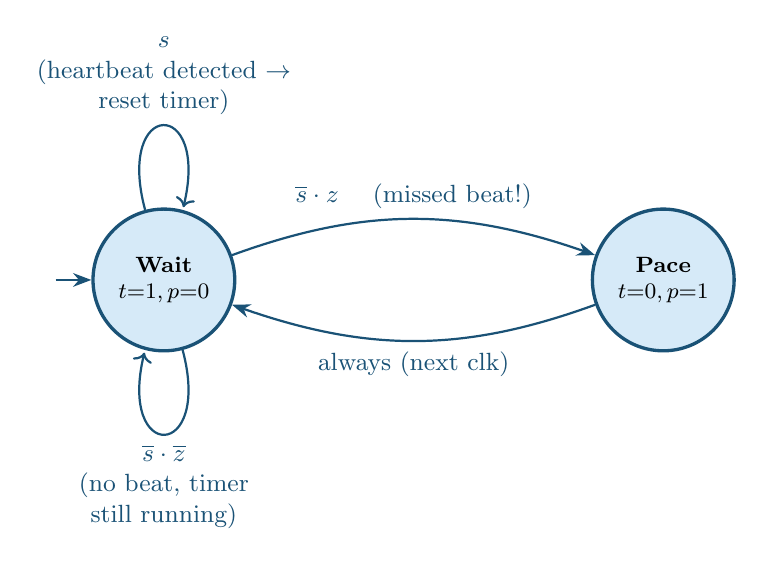
\begin{tikzpicture}[node distance=4.5cm]
  \node[fsm state, initial, minimum size=1.8cm] (wait) {\textbf{Wait} \\ $t{=}1, p{=}0$};
  \node[fsm state, right=of wait, minimum size=1.8cm] (pace) {\textbf{Pace} \\ $t{=}0, p{=}1$};
  
  \draw[fsm arrow] (wait) edge[loop above] node[above, align=center, font=\small]{$s$\\(heartbeat detected $\to$\\reset timer)} (wait);
  \draw[fsm arrow] (wait) edge[loop below] node[below, align=center, font=\small]{$\overline{s} \cdot \overline{z}$\\(no beat, timer\\still running)} (wait);
  \draw[fsm arrow] (wait) to[bend left=20] node[above, font=\small]{$\overline{s} \cdot z$ \quad (missed beat!)} (pace);
  \draw[fsm arrow] (pace) to[bend left=20] node[below, font=\small]{always (next clk)} (wait);
\end{tikzpicture}
\caption{Pacemaker controller FSM}
\label{fig:pacemaker}
\end{figure}

\subsection{How It Works}

\begin{enumerate}
  \item \textbf{Wait state} ($t{=}1, p{=}0$): Timer is running, no pacing.
  \begin{itemize}
    \item If heartbeat detected ($s{=}1$): Stay in Wait, reset timer --- heart is fine!
    \item If timer expires ($z{=}1$) without heartbeat ($s{=}0$): Heart missed a beat! $\to$ Go to Pace
  \end{itemize}
  \item \textbf{Pace state} ($p{=}1, t{=}0$): Send one electrical pulse.
  \begin{itemize}
    \item Immediately return to Wait on next clock edge.
  \end{itemize}
\end{enumerate}

\begin{important}[Safety-Critical Design]
  This is a \textbf{life-critical} FSM! A bug could harm a patient. This demonstrates why \textbf{formal FSM design} (not trial-and-error) is absolutely essential for safety-critical systems.
\end{important}

% ═══════════════════════════════════════════════════════
% SECTION 10: CHAPTER SUMMARY
% ═══════════════════════════════════════════════════════
\section{Chapter Summary \& Key Takeaways}

\begin{keypoint}[What We Learned]
  \begin{enumerate}[leftmargin=*]
    \item \textbf{Sequential circuits have state} --- they remember past inputs.
    \item \textbf{D flip-flop} is the robust bit-storage device; several together form a \textbf{register}.
    \item \textbf{FSM} is the formal model for sequential behavior (like Boolean equations are for combinational).
    \item The \textbf{5-step design process} systematically converts any FSM to a working circuit:
    \begin{enumerate}
      \item Capture FSM $\to$ 2A. Architecture $\to$ 2B. Encode $\to$ 2C. Truth Table $\to$ 2D. Logic
    \end{enumerate}
    \item \textbf{Glitching} can be solved via registered outputs or state-as-output encoding.
    \item We can now build the class of sequential circuits known as \textbf{controllers}.
  \end{enumerate}
\end{keypoint}

% ═══════════════════════════════════════════════════════
% SECTION 11: CHEAT SHEET
% ═══════════════════════════════════════════════════════
\section{Quick Reference Cheat Sheet}

\subsection{FSM Design Checklist}

\begin{description}[leftmargin=2.5cm, font=\bfseries]
  \item[Step 1:] Draw FSM state diagram
  \begin{itemize}
    \item Identify all states, inputs, outputs
    \item Draw transitions with conditions, mark initial state
  \end{itemize}
  \item[Step 2A:] Set up architecture: \texttt{inputs $\to$ [Comb Logic] $\to$ outputs}, with \texttt{[State Register]} below
  \item[Step 2B:] Encode states with unique binary codes
  \item[Step 2C:] Create truth table (inputs: state bits + FSM inputs; outputs: FSM outputs + next state bits)
  \item[Step 2D:] Derive Boolean equations, simplify, draw gates
\end{description}

\subsection{Common FSM Patterns}

\begin{table}[H]
\centering
\renewcommand{\arraystretch}{1.4}
\begin{tabular}{@{} l l l @{}}
  \toprule
  \textbf{Pattern} & \textbf{Use Case} & \textbf{Example} \\
  \midrule
  Counter & Do something for $N$ cycles & Laser timer \\
  Toggle & Alternate between two states & Clock divider \\
  Wait-Act & Wait for trigger, act, return & Pacemaker \\
  Sequence Detector & Detect input pattern & Security code \\
  \bottomrule
\end{tabular}
\end{table}

\subsection{Key Formulas}

\begin{align*}
  \text{Number of flip-flops needed} &= \lceil \log_2(\text{number of states}) \rceil \\[8pt]
  \text{2 states} \to 1~\text{FF} \quad&\quad \text{3--4 states} \to 2~\text{FFs} \\
  \text{5--8 states} \to 3~\text{FFs} \quad&\quad \text{9--16 states} \to 4~\text{FFs}
\end{align*}

% ═══════════════════════════════════════════════════════
% SECTION 12: PRACTICE PROBLEMS
% ═══════════════════════════════════════════════════════
\section{Practice Problems}

\subsection{Problem 1: 2-Cycle Delay}
Design an FSM that outputs $y=1$ exactly \textbf{2 clock cycles} after input $a$ becomes 1.

\begin{tip}[Hint]
  3 states: Wait, Delay1, Delay2. When $a=1$: Wait $\to$ Delay1 $\to$ Delay2 ($y{=}1$) $\to$ Wait.
\end{tip}

\subsection{Problem 2: Sequence Detector}
Design an FSM that outputs $z=1$ when it detects the input sequence \textbf{1, 0, 1} on input $w$.

\begin{tip}[Hint]
  4 states: $S_0$ (initial), Got1 (seen ``1''), Got10 (seen ``1,0''), Got101 (seen ``1,0,1'' $\to$ $z{=}1$). Consider overlapping sequences!
\end{tip}

\subsection{Problem 3: Vending Machine}
A vending machine accepts nickels ($N$) and dimes ($D$). It dispenses a drink (output $\text{dispense}=1$) when 15 cents or more is inserted. Design the FSM.

\begin{tip}[Hint]
  States represent accumulated cents: $S_0$ (0\textcent), $S_5$ (5\textcent), $S_{10}$ (10\textcent), $S_{15}$ (15+\textcent, dispense).
\end{tip}

\vfill
\begin{center}
  \color{gray}\rule{0.5\textwidth}{0.5pt}\\[6pt]
  {\small\textit{Source: Frank Vahid, Digital Design, Chapter 3 --- Sequential Logic Design: Controllers}}\\[4pt]
  {\small\textbf{Key Takeaway:} FSMs provide a formal, systematic way to design sequential circuits. Always use the 5-step process --- never guess!}
\end{center}

\end{document}
